\chapter{Implementación}
\label{ch:implementacion}


\insertminitoc
\parindent0pt


\section{Diseño de la Solución tecnológica}
El diseño de la solución tecnológica para el sistema \textit{Parental AI Shield} establece la estructura técnica y conceptual orientada a la protección proactiva del menor mediante el análisis automático de contenido. A diferencia de los sistemas tradicionales basados en la nube, este diseño se fundamenta en el \textbf{procesamiento en el borde} (\textit{Edge Computing}), donde la detección de amenazas ocurre directamente en el dispositivo móvil. Este método posibilita representar la actividad digital del menor como un flujo de eventos multimodales, capturando tanto la información visual de la pantalla como la semántica de las interacciones textuales para identificar riesgos de \textit{sexting}, \textit{grooming} o acoso.

La estructura del sistema se organiza bajo un \textbf{diseño modular}, integrando cuatro componentes principales:
\begin{itemize}
    \item \textbf{Captura y normalización de eventos de accesibilidad:} Este módulo actúa como el sensor primario del sistema. Utiliza la \gls{api} de accesibilidad de Android para extraer de forma no intrusiva capturas de pantalla (\textit{bitmaps}) y nodos de texto (\textit{AccessibilityNodeInfo}) de aplicaciones externas. Los datos son normalizados y escalados para ser compatibles con los requisitos de entrada de los modelos de Inteligencia Artificial.
    \item \textbf{Motor de inferencia inteligente bimodal:} Es el núcleo analítico donde residen los modelos de \textit{Machine Learning} (desarrollados en Python y optimizados mediante Google Colab). Este módulo ejecuta inferencias paralelas: un modelo de visión artificial para clasificar contenido visual \gls{nsfw} y un modelo de Procesamiento de Lenguaje Natural (\gls{nlp}) para detectar patrones de acoso en los chats.
    \item \textbf{Persistencia y gestión de evidencias (Bitácora):} Diseñado para garantizar la integridad y privacidad de la información. Este componente utiliza una base de datos local SQLite para registrar las alertas y gestiona el almacenamiento físico de las capturas de pantalla en directorios protegidos del sistema operativo, asegurando que las evidencias no sean accesibles para otras aplicaciones o usuarios ajenos al tutor.
    \item \textbf{Dashboard de supervisión parental:} Desarrollado con el framework moderno Jetpack Compose, este módulo permite la visualización y auditoría de los resultados. Presenta de forma cronológica las alertas detectadas, permitiendo al tutor legal revisar las evidencias (imágenes y textos de riesgo) y tomar decisiones informadas sobre la seguridad digital del menor.
\end{itemize}

Esta arquitectura modular asegura la \textbf{mantenibilidad y escalabilidad}, permitiendo que en el futuro se incorporen nuevos modelos de \gls{ia} para detectar otros riesgos (como apuestas o fraudes) sin alterar la lógica de captura o persistencia.

\subsection{Arquitectura general del sistema}
La arquitectura se estructura en cuatro niveles interconectados, diseñados para garantizar un flujo de información eficiente desde la captura hasta la presentación de alertas:\\


\begin{itemize}
    \item \textbf{Capa de adquisición de datos:} Constituye el punto de contacto con el sistema operativo Android. Gestiona los permisos de accesibilidad y filtra los eventos relevantes para evitar el procesamiento de aplicaciones bancarias o de ingreso de contraseñas, protegiendo la privacidad sensible del usuario.\\
    \item \textbf{Capa de procesamiento de Inteligencia Artificial:} En este nivel se integran los modelos exportados en formato TensorFlow Lite (.tflite). Las tareas principales incluyen:\\
    \begin{itemize}
        \item Redimensionamiento y conversión de color de fotogramas mediante librerías de procesamiento de imagen.
        \item Tokenización y limpieza semántica de las cadenas de texto capturadas en redes sociales.
        \item Ejecución de inferencia asíncrona mediante el uso de \textit{Kotlin Coroutines}, lo que permite que el análisis ocurra sin afectar la fluidez del dispositivo del menor.
        \item Clasificación probabilística y detonación de eventos según los umbrales de riesgo preconfigurados.
    \end{itemize}
    \item \textbf{Capa de persistencia segura:} Esta capa abstrae la complejidad del almacenamiento. Utiliza \textit{Room} o \textit{SQLiteOpenHelper} para gestionar los registros relacionales y rutinas de cifrado o aislamiento de archivos para las capturas de pantalla guardadas en el almacenamiento interno privado de la aplicación.\\
    \item \textbf{Capa de presentación de alertas:} Es el punto de interacción con el tutor legal. Transforma los datos crudos de la base de datos en información útil, categorizando las alertas por severidad y tipo (visual o textual), facilitando una respuesta rápida ante posibles situaciones críticas.\\\\\\\\\\\\\\
\end{itemize}

\begin{figure}[!htbp]
    \centering
    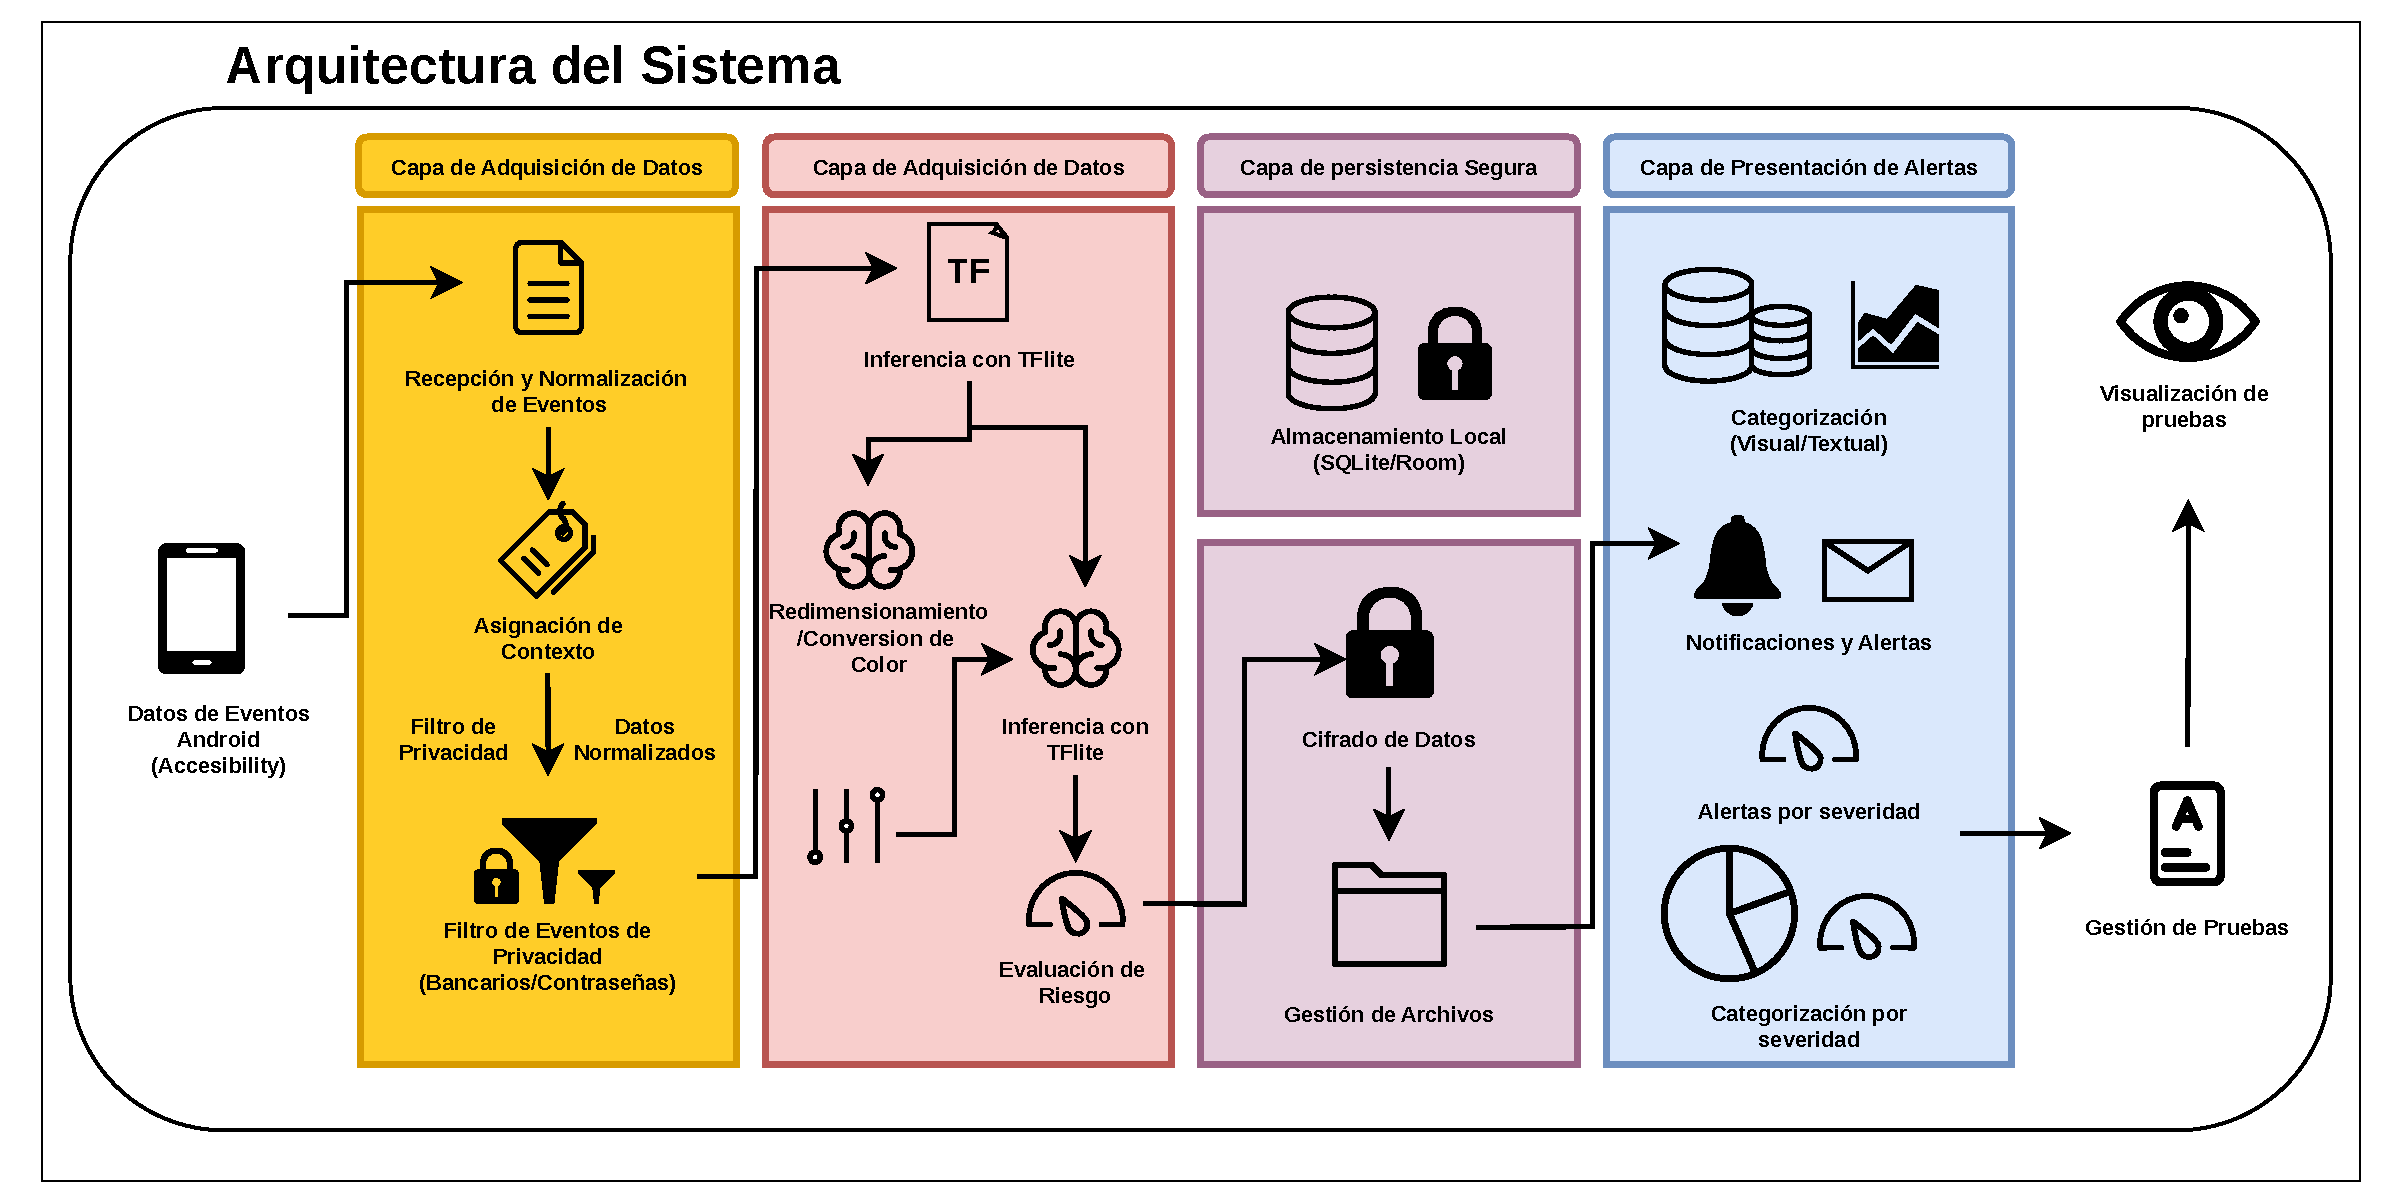
\includegraphics[width=1\linewidth]{Figures/arquitectura de sistema.pdf}
    \caption[Arquitectura del Sistema de Control Parental Basado en Aprendizaje Automático orientado a la Protección Infantil en la Era Digital]{Arquitectura del Sistema de Control Parental Basado en Aprendizaje Automático orientado a la Protección Infantil en la Era Digital. Fuente: Elaboración propia.}
    \label{fig:figure-arquitectura-sistema}
\end{figure}

\section{Flujo de procesos}
\subsection{Flujo de procesos del sistema}
El recorrido operativo del sistema, conocido como flujo de procesos, se encarga de convertir la información reunida del dispositivo del menor —datos sobre capturas visuales, texto detectado y probabilidades de riesgo— en hallazgos que ayudan a los tutores legales a tomar decisiones de supervisión informadas, tanto a nivel preventivo como correctivo. Esta conversión no es directa; sigue un ciclo estricto y permanente de monitoreo y análisis. El flujo cuenta con seis fases clave, estructuradas en un circuito que transita desde la captura inicial hasta la presentación de evidencias en el panel de control, permitiendo una mejora continua en la precisión del sistema:

\begin{itemize}
    \item \textbf{Captura de eventos mediante servicios de accesibilidad:} Recolección no intrusiva de fotogramas de pantalla y árboles de nodos de texto de aplicaciones externas.
    \item \textbf{Preprocesamiento bimodal:} Normalización de mapas de bits y tokenización de cadenas de texto para su compatibilidad con los motores de \gls{ia}.
    \item \textbf{Inferencia de Inteligencia Artificial:} Ejecución local de los modelos de visión artificial (\gls{nsfw}) y procesamiento de lenguaje natural (acoso/grooming).
    \item \textbf{Clasificación y evaluación de umbrales:} Determinación de la severidad del riesgo detectado basándose en los índices de probabilidad de los modelos.
    \item \textbf{Persistencia en Bitácora de evidencias:} Registro cifrado de alertas y almacenamiento de capturas en la base de datos SQLite local del dispositivo.
    \item \textbf{Visualización en el Dashboard parental:} Presentación de resultados y estadísticas críticas al tutor para la retroalimentación y toma de acciones.
\end{itemize}

\begin{figure}
    \centering
    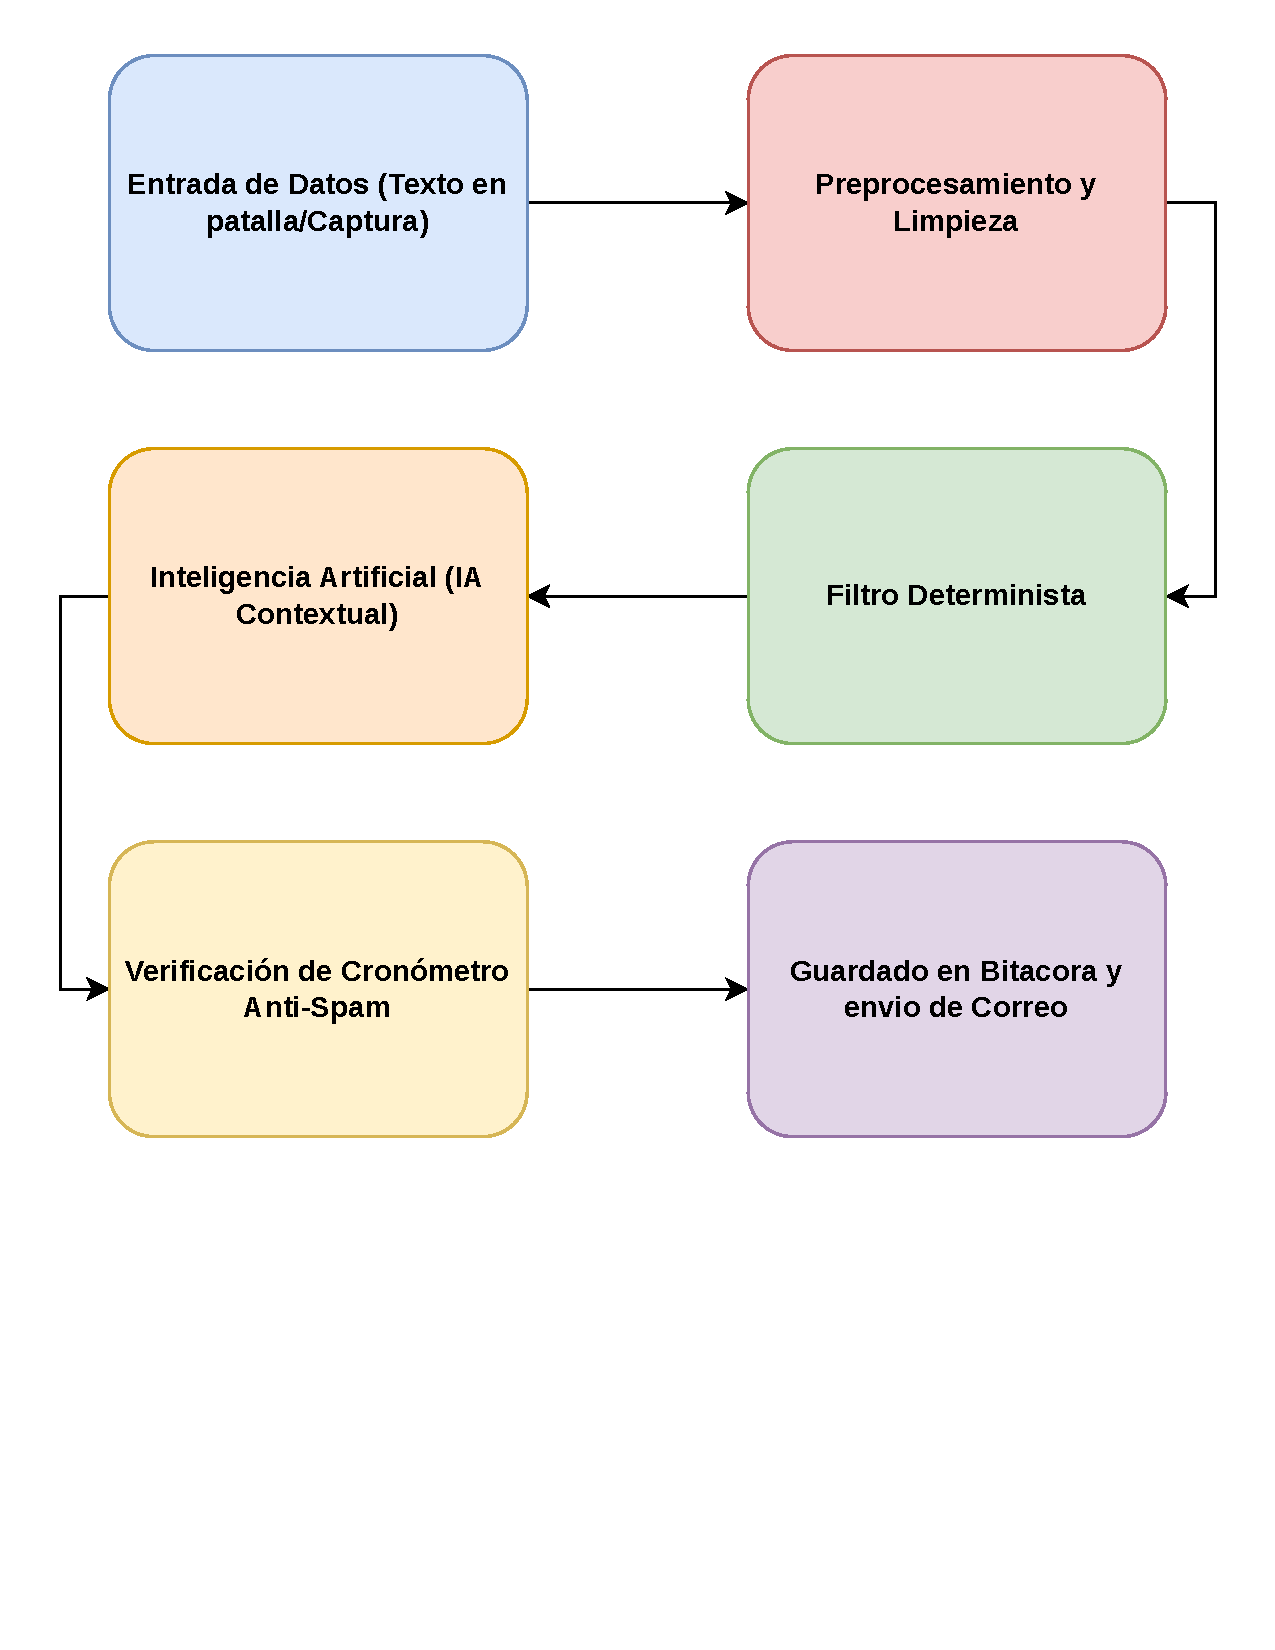
\includegraphics[width=0.9\linewidth]{Figures/diagramaProceso.drawio.pdf}
    \caption[Flujo de procesos del sistema de monitoreo inteligente para protección infantil]{Flujo de procesos unificado del Sistema de Monitoreo Inteligente para Protección Infantil, integrando análisis de texto contextual (\gls{nlp}) y detección visual. Fuente: Elaboración propia.}
    \label{fig:figure-flujo-procesos}
\end{figure}
\section{Implementación del Sistema de Monitoreo y Análisis}

\subsection{Preparación y curación del dataset de entrenamiento}
El desarrollo del motor de inteligencia artificial comenzó con la recopilación y estructuración de un dataset bilingüe (español e inglés) especializado en riesgos digitales infantiles. A diferencia de los modelos genéricos, los datos se categorizaron en dos clases fundamentales para el entrenamiento:
\begin{itemize}
\item \textbf{Clase 0 (Seguro/SFW):} Incluye interacciones cotidianas, consultas académicas y, crucialmente, etiquetas de interfaz de usuario (\gls{ui}) capturadas de navegadores y redes sociales (ej. "Search or type URL", "Web Libros Vuelos").
\item \textbf{Clase 1 (Riesgo/\gls{nsfw}):} Compuesta por indicadores de \textit{grooming}, ciberacoso, contenido explícito y tácticas de manipulación psicológica (ej. "es nuestro secreto", "manda fotos sin ropa").
\end{itemize}

El proceso de preparación incluyó una fase crítica de limpieza y normalización en la que se eliminaron tildes, caracteres especiales y se estandarizó el texto a minúsculas. Asimismo, se aplicó una técnica de \textbf{mapeo de casos límite} (\textit{edge-case mapping}) para desensibilizar al modelo ante falsos positivos comunes en videojuegos como Roblox o búsquedas biológicas, garantizando que el sistema aprenda a diferenciar el contexto y no solo palabras aisladas.

\subsection{Desarrollo del modelo de análisis basado en Deep Learning}
El modelo predictivo fue desarrollado en el entorno de Google Colab, utilizando el ecosistema de TensorFlow y Keras para la construcción de redes neuronales. El desarrollo se organizó en tres fases técnicas:

\begin{itemize}
\item \textbf{Arquitectura del modelo y procesamiento de lenguaje natural (\gls{nlp}):} Se implementó una red neuronal profunda con una capa de embedding para la representación vectorial de las palabras y una capa de \textbf{Convolución 1D (Conv1D)}. Esta elección técnica permite que la \gls{ia} analice bloques de palabras consecutivas (n-gramas), facilitando la comprensión del contexto gramatical.
\item \textbf{Entrenamiento y optimización local (\gls{tflite}):} Una vez validada la precisión del modelo en la nube, se procedió a su conversión al formato \textbf{TensorFlow Lite}. Este paso es esencial para permitir la ejecución de la \gls{ia} directamente en el dispositivo móvil del menor (\textit{on-device computing}), garantizando la privacidad de los datos al no requerir el envío de conversaciones a servidores externos para su análisis.
\item \textbf{Integración del Servicio de Accesibilidad en Android:} La implementación en el dispositivo se realizó mediante un servicio de accesibilidad en Kotlin, configurado para interceptar eventos de ventana. Este componente actúa como el puente entre la interfaz de usuario y el modelo de \gls{ia}, extrayendo el texto en tiempo real y disparando capturas de pantalla silenciosas únicamente cuando se detecta un umbral de riesgo superior al 60 porciento.
\end{itemize}

\subsection{Gestión de evidencias y visualización de resultados}
Para asegurar que la información sea útil para el tutor legal, se desarrolló una interfaz de monitoreo y un sistema de alertas automatizado que incluye:
\begin{itemize}
\item \textbf{Bitácora de evidencias interactiva:} Un registro local basado en una arquitectura de tarjetas expandibles. Al detectar una alerta, el sistema almacena el fragmento de texto, la aplicación de origen y la captura de pantalla vinculada. La interfaz permite al tutor expandir la evidencia visual para un análisis detallado mediante un visor modal de alta resolución.
\item \textbf{Sistema de notificación asíncrona:} Integración con Firebase para el envío de reportes mediante correo electrónico. Para optimizar la seguridad y el almacenamiento, las capturas de pantalla se procesan mediante serialización en \textbf{Base64}, adjuntándose directamente al cuerpo del mensaje sin necesidad de subidas a nubes públicas.
\item \textbf{Mecanismo de protección de privacidad:} Implementación de un "Escudo de Monitoreo" que desactiva el escaneo cuando la aplicación propia está en primer plano, evitando bucles de detección y garantizando que el tutor pueda revisar los registros sin activar nuevas alertas.
\end{itemize}

\subsection{Integración con el entorno de ejecución y monitoreo}
Una vez desarrollado y validado el modelo de análisis contextual, este se integró con el \textbf{Servicio de Accesibilidad de Android}, una herramienta de bajo nivel que permite interactuar con la capa de interfaz de usuario de cualquier aplicación instalada. Esta integración permitió capturar en tiempo real las condiciones de uso del dispositivo y evaluar cómo las predicciones del modelo influyen en la detección de riesgos bajo distintos escenarios de interacción. El proceso se llevó a cabo en las siguientes etapas: \

\textbf{Mapeo del entorno de interfaz de usuario (\gls{ui})} \
Se implementó un algoritmo de escaneo de nodos (\textit{AccessibilityNodeInfo}) que extrae de forma recursiva la estructura de la ventana activa. Para ello, se identificaron los elementos clave de la pantalla, como campos de texto, descripciones de imágenes y estados de navegación. En áreas de baja relevancia (como botones de sistema), el escaneó se simplificó; sin embargo, en aplicaciones críticas como navegadores web y mensajería, identificadas mediante el análisis de riesgos previo, se conservó una extracción de datos de alta precisión. \

\textbf{Definición de flujos de eventos y datos} \
Se definieron flujos de datos basados en los tipos de interacción del menor (chats, búsquedas en Google, navegación en redes sociales). Estos flujos fueron calibrados utilizando los registros seguros e inseguros previamente estructurados en el dataset. El sistema fue diseñado para ignorar el "ruido visual" de las interfaces y centrarse únicamente en el contenido semántico generado por el usuario. \

\textbf{Monitoreo y control de riesgos en tiempo real} \
Se ejecutaron pruebas de estrés considerando distintos escenarios de uso: navegación en modo incógnito, uso de aplicaciones de juegos (ej. Roblox), y conversaciones de mensajería con lenguaje ambiguo. El servicio permitió registrar métricas de rendimiento como:
\begin{itemize}
\item tiempo de latencia de la inferencia (en milisegundos),
\item precisión del umbral de riesgo detectado,
\item efectividad en la captura de pantalla ante eventos críticos,
\item y consumo de recursos (\gls{cpu}/Batería) del servicio en segundo plano.
\end{itemize}
Toda la información fue almacenada localmente en una base de datos SQLite y exportada a Firebase para su análisis remoto por parte del tutor. \

\textbf{Análisis de escenarios de riesgo} \
Los datos recolectados se procesaron para comparar el desempeño de la aplicación bajo diferentes configuraciones de sensibilidad del modelo. A partir de este análisis fue posible:
\begin{itemize}
\item identificar aplicaciones con mayor probabilidad de generar falsos positivos,
\item evaluar la sensibilidad del sistema ante cambios en el lenguaje del menor,
\item comparar la eficiencia de la detección entre el filtro directo y la \gls{ia} contextual,
\item y examinar cómo la privacidad local influye en la confianza del sistema.
\end{itemize}
Los resultados permitieron validar la robustez del sistema en un entorno de ejecución real, basándose en métricas de confianza de Machine Learning y comportamiento del usuario monitorizado.

\subsection{Entorno de desarrollo y herramientas utilizadas}
El desarrollo completo del sistema se llevó a cabo utilizando los siguientes recursos tecnológicos:

\begin{itemize}
\item Lenguaje de programación: Kotlin 1.9 (Android) y Python 3.11 (\gls{ia})
\item Entornos de trabajo: Android Studio Jellyfish y Google Colab
\item Arquitectura de \gls{ia}: TensorFlow Lite (Inferencia local)
\item Gestión de datos y nube: SQLite (Local) y Firebase Firestore (Remoto)
\end{itemize}

Equipo de desarrollo: PC MSI KATANA 15 B13V con procesador Intel Core i7-13700H, 16GB de \gls{ram} y sistema operativo Windows 11. 
Estos elementos permitieron un flujo de trabajo eficiente, combinando potencia de cálculo local y recursos en la nube para la 
ejecución de tareas de análisis y simulación intensivas.


\subsection{Validación inicial del sistema}
El proceso de implementación incluyó la realización de pruebas unitarias y de integración utilizando diferentes volúmenes de datos textuales y diversas configuraciones de interfaz de usuario. El sistema demostró ser capaz de procesar flujos de texto capturados por el servicio de accesibilidad sin errores de desbordamiento de memoria y de generar reportes automáticos de riesgo mediante el servicio de notificaciones asíncronas de Firebase.

\section{Pruebas y resultados preliminares}

\subsection{Análisis del lenguaje de riesgo mediante Procesamiento de Lenguaje Natural (\gls{nlp})}
El análisis de los patrones de comunicación y detección de contenido sensible se llevó a cabo mediante el uso del lenguaje de programación \textbf{Python} en el entorno de \textbf{Google Colaboratory}. La metodología implementada se basó en el modelado de secuencias de texto mediante redes neuronales convolucionales (Conv1D) a partir de un dataset especializado en seguridad infantil. Para ello, se emplearon las librerías especializadas \textbf{TensorFlow} y \textbf{Keras}, que facilitaron tanto el entrenamiento de los \textbf{Word Embeddings} (representaciones vectoriales de las palabras) como la generación de la estructura lógica del modelo.

Tras el análisis semántico, se logró la identificación de los "disparadores críticos" (\textit{triggers}) del sistema. A estos se les asignó una alta ponderación debido a su significación contextual: la combinación de ciertos términos (ej. nombres de órganos, verbos de acción y peticiones de secreto) genera un impacto sustancial en el nivel de confianza de la alerta, permitiendo que el modelo diferencie entre una conversación trivial y una posible amenaza de \textit{grooming} o ciberacoso. Este hallazgo subraya la capacidad del modelo para evaluar la vulnerabilidad del menor ante patrones de lenguaje manipulativo.

\subsection{Preprocesamiento y Vectorización Avanzada}
Una de las mayores dificultades en el análisis de texto en español es la variabilidad ortográfica. Para asegurar la coherencia entre el entrenamiento en la nube y la ejecución en el dispositivo móvil, se implementó una función de \textbf{Estandarización Personalizada} (\textit{Custom Standardization}).

Esta función realiza un proceso de limpieza profunda mediante expresiones regulares (Regex), transformando caracteres con tildes y diéresis a sus versiones base (ej. 'á' a 'a'). Esto reduce la dispersión del vocabulario, permitiendo que la \gls{ia} reconozca palabras de riesgo independientemente de si el usuario utilizó la acentuación correcta. Posteriormente, se utilizó una capa de \textbf{TextVectorization} con un vocabulario de 2,000 tokens y una longitud máxima de 50 palabras, transformando las cadenas de texto en tensores numéricos procesables por la red neuronal.

\subsection{Arquitectura del Modelo de Red Neuronal (\gls{cnn} + \gls{nlp})}
El motor de detección se basa en una arquitectura de Aprendizaje Profundo (\textit{Deep Learning}) diseñada para ser ligera y altamente sensible al contexto. El modelo se estructuró en cinco capas fundamentales:

\begin{itemize}
\item \textbf{Capa de Embedding (32 dimensiones):} Transforma los números enteros del vectorizador en vectores densos. En este espacio vectorial, las palabras con significados similares ej. "secreto" y "ocultar" se agrupan matemáticamente, permitiendo a la \gls{ia} entender semántica básica.
\item \textbf{Capas de Dropout (0.4):} Se insertaron capas de "abandono" que desactivan aleatoriamente el 40 porciento de las neuronas durante el entrenamiento. Esta es una técnica crítica de regularización para evitar el \textit{Overfitting} (sobreajuste), obligando a la red a aprender patrones generales de riesgo en lugar de memorizar frases específicas del dataset.
\item \textbf{Capa Convolucional 1D (Conv1D):} Es el núcleo del análisis de contexto. Utiliza un \textit{kernel} de tamaño 3, lo que significa que la \gls{ia} analiza "n-gramas" o grupos de tres palabras consecutivas. Esto permite detectar estructuras de manipulación como "no + digas + nada".
\item \textbf{GlobalMaxPooling1D:} Esta capa actúa como un filtro de intensidad. Recorre todo el texto analizado y extrae únicamente la señal de peligro más fuerte detectada, ignorando el resto del texto inofensivo para reducir el ruido.
\item \textbf{Capa de Salida (Sigmoid):} Utiliza una función de activación sigmoidea para comprimir el resultado en un valor entre 0 y 1, representando la probabilidad porcentual de riesgo.
\end{itemize}

\begin{figure}[H]
    \centering
    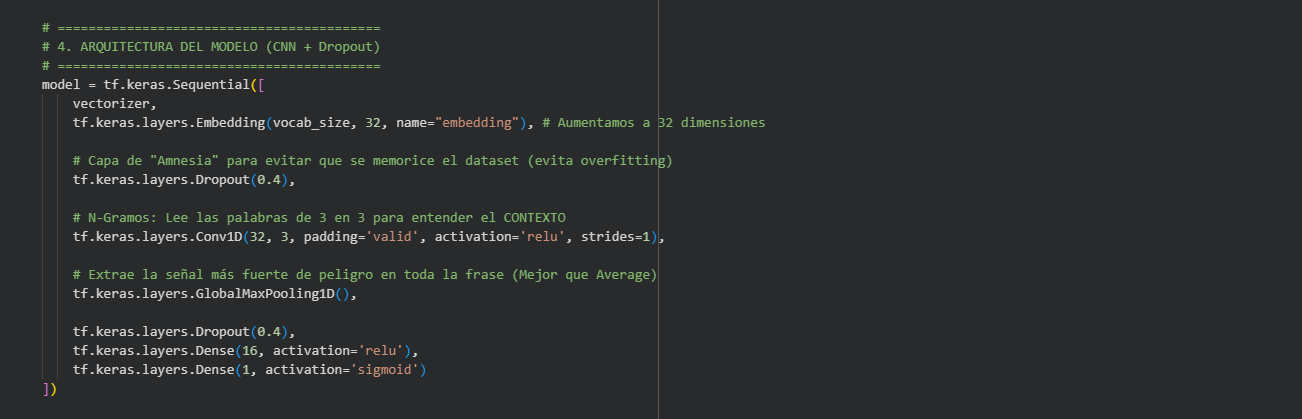
\includegraphics[width=1\linewidth]{Figures/codigoCNN.png}
    \caption[Implementación detallada de la vectorización avanzada y arquitectura Conv1D]{Implementación detallada de la vectorización avanzada y arquitectura Conv1D para detección de riesgo infantil. Fuente: Elaboración propia.}
    \label{fig:figure-codigo-entrenamiento}
\end{figure}

\subsection{Estrategia de Entrenamiento y Optimización}
Para garantizar la robustez del modelo, se implementó un proceso de entrenamiento supervisado utilizando el optimizador \textbf{Adam} y la función de pérdida \textbf{Binary Crossentropy}, estándar para problemas de clasificación binaria.

Un aspecto innovador de esta implementación es el uso de \textbf{Early Stopping} (Frenado Temprano). Se configuró un monitor con una paciencia de 10 épocas para supervisar la pérdida en el set de validación. Si la \gls{ia} deja de mejorar su capacidad de generalización durante 10 iteraciones, el entrenamiento se detiene automáticamente y se restauran los mejores pesos. Esto no solo optimiza el tiempo de cómputo, sino que garantiza que el modelo final sea el más equilibrado para detectar riesgos en situaciones reales sin generar falsas alarmas.

\begin{figure}[H]
    \centering
    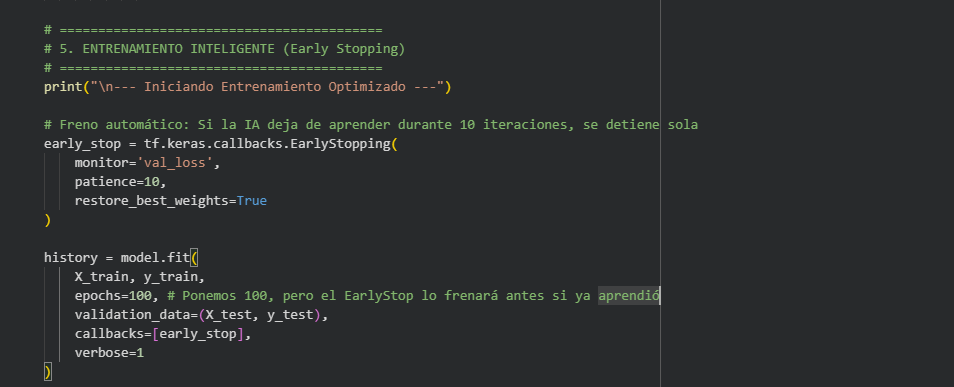
\includegraphics[width=1\linewidth]{Figures/EarlyStop.png}
    \caption[Configuración del algoritmo de Early Stopping para la optimización del entrenamiento]{Configuración del algoritmo de Early Stopping encargado de monitorear la pérdida de validación y prevenir el sobreajuste del modelo. Fuente: Elaboración propia.}
    \label{fig:figure-early-stopping}
\end{figure}

\subsection{Procesamiento y Curación del Dataset Visual}
El desarrollo de los módulos de visión artificial requirió una fase de saneamiento de datos para asegurar la integridad de las imágenes de entrenamiento. Se implementó un algoritmo de escaneo profundo utilizando la librería \textbf{OpenCV} y el decodificador nativo de \textbf{TensorFlow} para realizar una purga de archivos corruptos o en formatos incompatibles, como imágenes en espacio de color CMYK o archivos JPEG truncados. Este proceso garantiza que los tensores generados durante el entrenamiento sean válidos y no interrumpan el flujo de aprendizaje del modelo.

\subsection{Arquitectura de Visión Artificial mediante Transfer Learning}
Para la detección de contenido inapropiado, se optó por una arquitectura basada en \textbf{MobileNetV2}, un modelo de red neuronal convolucional optimizado para dispositivos móviles. El proceso de construcción se dividió en dos etapas técnicas fundamentales:

\begin{itemize}
    \item \textbf{Transfer Learning (Aprendizaje por Transferencia):} Se utilizó un modelo base pre-entrenado con el dataset ImageNet, congelando sus 154 capas iniciales para conservar la capacidad de detección de formas y texturas básicas. Sobre esta base, se añadieron capas personalizadas de \textbf{GlobalAveragePooling2D} y \textbf{Dropout} al 20\% para prevenir el sobreajuste.
    \item \textbf{Ajuste Fino (Fine-Tuning):} En una segunda fase, se descongelaron las capas superiores del modelo y se realizó un re-entrenamiento con una tasa de aprendizaje extremadamente baja ($1 \times 10^{-5}$). Esto permitió que la \gls{ia} especializara sus neuronas de alto nivel en la identificación de patrones específicos de contenido \gls{nsfw} y material explícito sin destruir el conocimiento previo del modelo.
\end{itemize}

\subsection{Detección Multimodelo: Contenido Explícito y Violencia/Gore}
La robustez del sistema se complementó mediante la implementación de una lógica de entrenamiento idéntica para un segundo modelo especializado en la detección de \textbf{Violencia y material Gore}. Al replicar la arquitectura de MobileNetV2 y la técnica de \textit{Fine-Tuning}, el sistema adquirió la capacidad de clasificar imágenes en categorías de riesgo adicionales, permitiendo que el servicio de monitoreo en Android dispare alertas diferenciadas según la naturaleza de la amenaza visual detectada.

\subsection{Optimización de Inferencia y Cuantización (Edge AI)}
Para que ambos modelos de visión pudieran ejecutarse en tiempo real sin agotar los recursos del dispositivo móvil, se aplicó un proceso de \textbf{Cuantización de Pesos} mediante \textit{TFLiteConverter}. Esta técnica convierte los pesos matemáticos de punto flotante de 32 bits a formatos más compactos, reduciendo drásticamente el peso del archivo final (\textit{.tflite}) y permitiendo una ejecución fluida en la \textbf{GPU} o \textbf{\gls{npu}} del celular.\\\\

\begin{figure}[H]
    \centering
    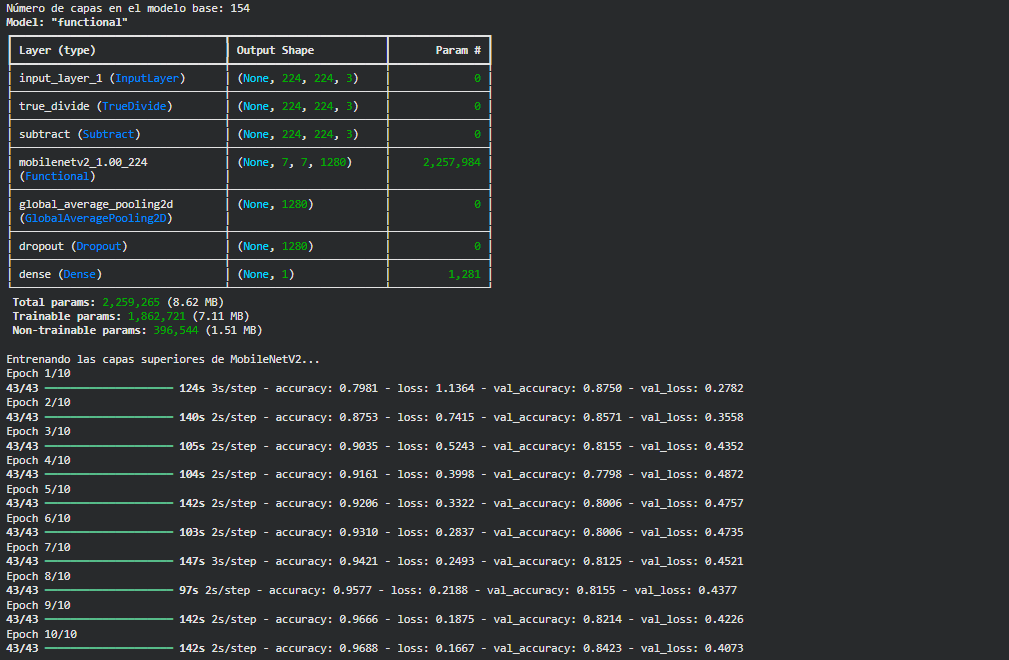
\includegraphics[width=1\linewidth]{Figures/entrenamientoImagens.png}
    \caption[Fase de ajuste fino y métricas de precisión del modelo de visión]{Métricas de entrenamiento durante la fase de Fine-Tuning para la optimización del modelo de visión artificial. Fuente: Elaboración propia.}
    \label{fig:figure-entrenamiento-vision}
\end{figure}

\subsection{Pruebas de monitoreo en el entorno Android}
La evaluación inicial de la aplicación se llevó a cabo utilizando escenarios de uso real, los cuales se construyeron a partir de la interacción con navegadores (Google Chrome) y aplicaciones de mensajería. Como parte del proceso de refinamiento metodológico, fue necesaria la modificación y ampliación de los filtros de limpieza en el código Kotlin, debido a una generación inconsistente de alertas provocada por el "ruido visual" de la interfaz de usuario de Chrome (ej. botones de "Vuelos", "Finanzas" e imágenes del modo \gls{ia}).\\

Posteriormente, se procedió a la ejecución de pruebas de estrés sobre la captura de evidencias visuales. Este proceso permitió cuantificar y mapear la precisión del sistema, logrando identificar y especificar numéricamente el nivel de confianza (porcentaje de riesgo) ante búsquedas explícitas. Esta fase resultó crucial para la validación y la calibración del modelo \gls{tflite}, asegurando que la activación de la cámara silenciosa y el guardado en la bitácora ocurran únicamente ante eventos de alta probabilidad de riesgo, minimizando así la intrusión en la privacidad rutinaria del menor.\\

\begin{figure}[H]
\centering
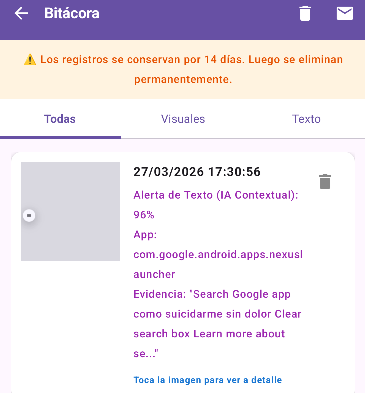
\includegraphics[width=1\linewidth]{Figures/bitacoraAndroid.png}
\caption[Interfaz de la bitácora con registro de evidencias]{Visualización de alertas capturadas y validación de evidencias en la bitácora. Fuente: Elaboración propia.}
\label{fig:figure-bitacora-android}
\end{figure}

\subsection{Pruebas de estrés y rendimiento del sistema}

Se llevaron a cabo pruebas de sensibilidad incrementales con el propósito de evaluar la resiliencia y la capacidad de respuesta del servicio de monitoreo frente a diversos escenarios de flujo intensivo de datos. Específicamente, se modelaron dos condiciones críticas de operación:

\begin{itemize}
\item \textbf{Escenario de Uso Intensivo (Proyectado):} Se aplicó un incremento en la frecuencia de entrada de texto, simulando un comportamiento de mensajería instantánea de alta velocidad (aprox. 20 mensajes por minuto). Esto permitió evaluar la estabilidad del modelo \textit{on-device} ante ráfagas de datos.
\item \textbf{Escenario de Saturación y Concurrencia:} Se simuló una etapa de carga extrema donde el volumen de texto se duplicó y se procesaron capturas de pantalla de forma simultánea. El objetivo fue verificar la gestión de memoria \gls{ram} del dispositivo y asegurar que el hilo de ejecución de la \gls{ia} no interfiriera con la fluidez del sistema operativo Android.
\end{itemize}

Estas simulaciones resultaron esenciales para determinar los umbrales de servicio del modelo \gls{tflite}, identificar posibles fugas de memoria (\textit{memory leaks}) en el servicio de accesibilidad y garantizar un desempeño óptimo del sistema ante incrementos significativos en la actividad digital del menor.

\begin{figure}[H]
\centering
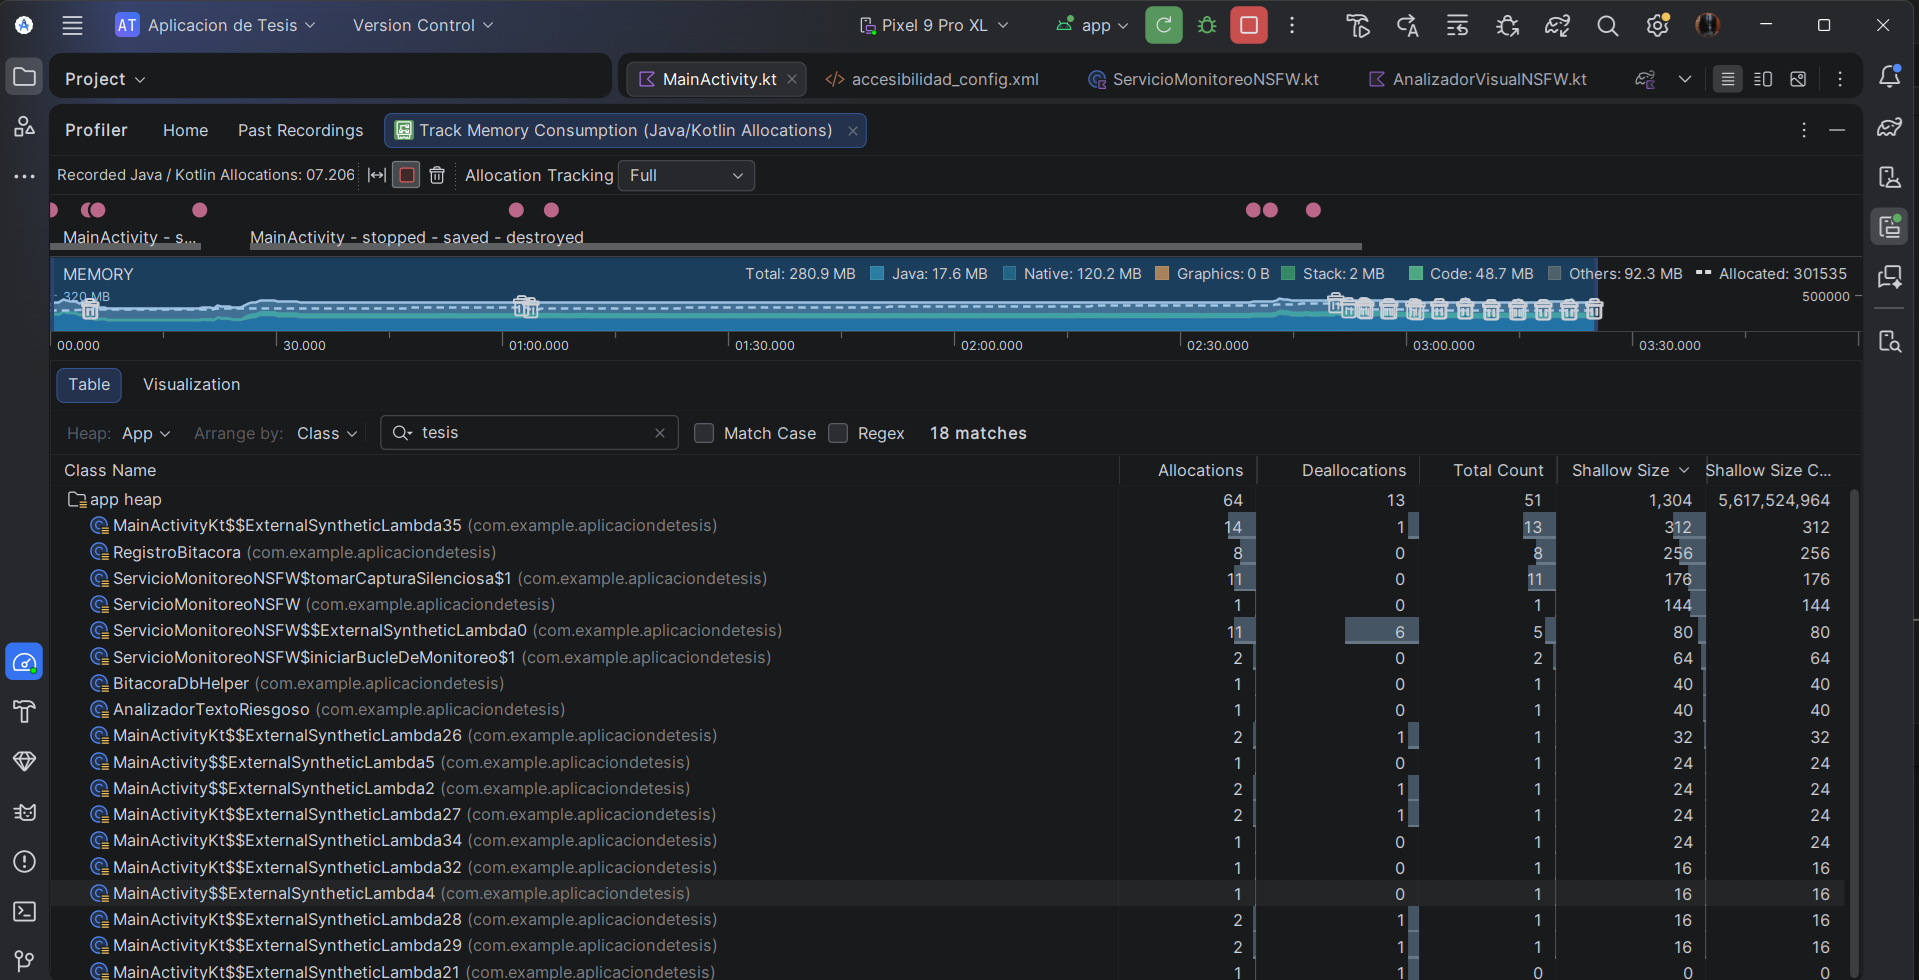
\includegraphics[width=1\linewidth]{Figures/androidProfiller.png}
\caption[Monitoreo de recursos en Android Profiler]{Monitoreo de consumo de \gls{cpu} y memoria durante las pruebas de carga en Android Profiler. Fuente: Elaboración propia.}
\label{fig:figure-android-profiler}
\end{figure}

